\documentclass{standalone}
\usepackage{tikz}
\usetikzlibrary{patterns, positioning}


\begin{document}
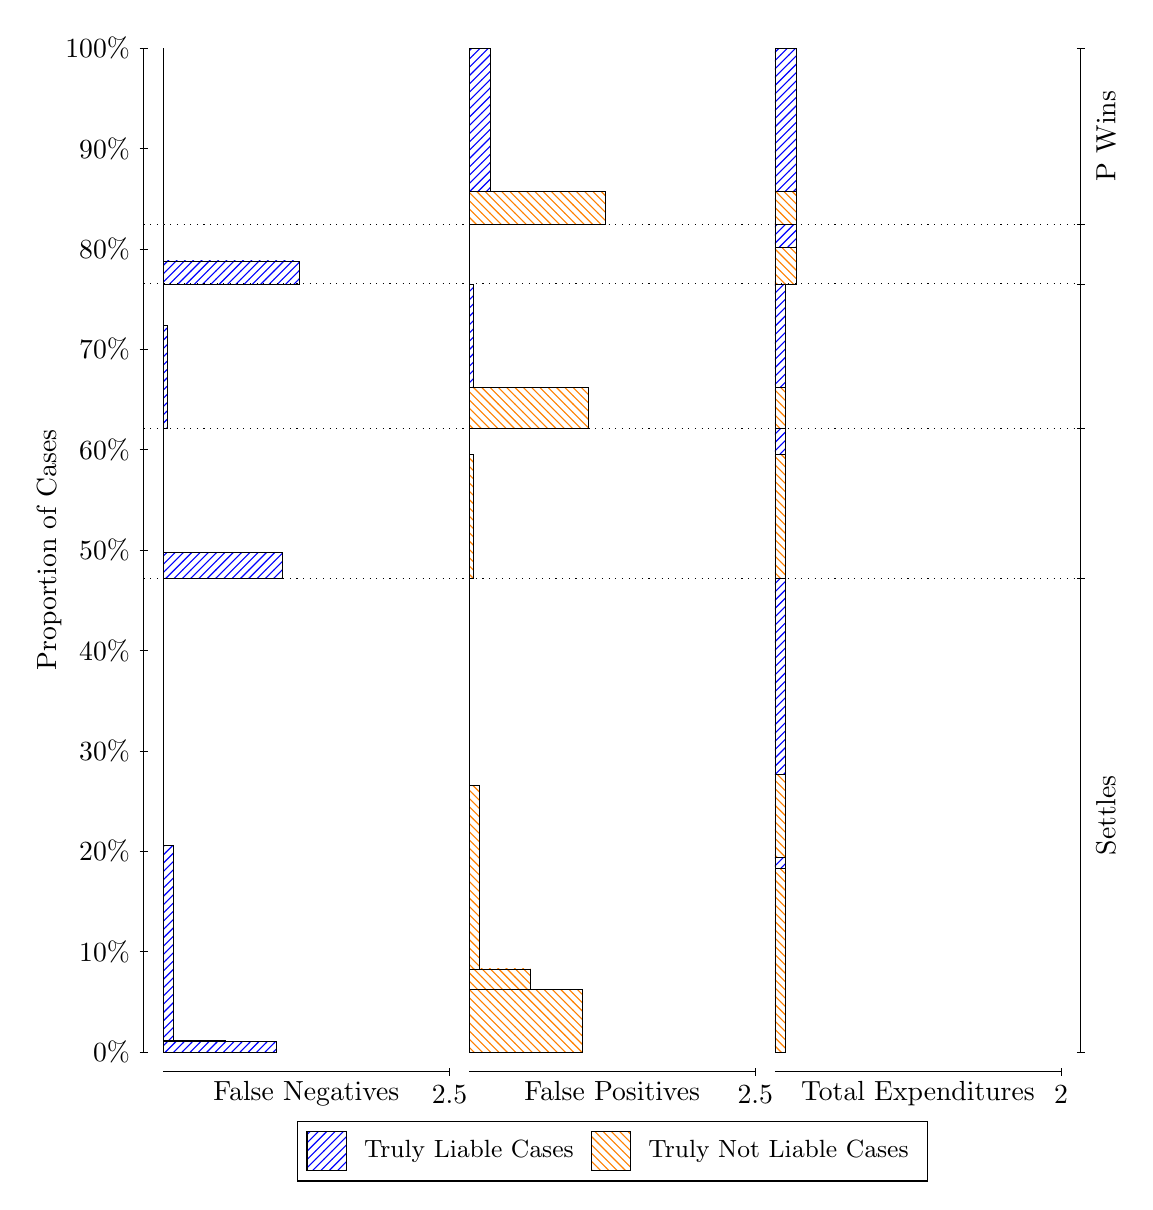
\begin{tikzpicture}
\draw[black, very thin] (1.5,1.75) -- (1.5,14.5);
\node[rotate=90, text=black, anchor=center] at (0.3, 8.125) {Proportion of Cases};
\draw[black, very thin] (1.45,1.75) -- (1.55,1.75);
\node[text=black, anchor=east] at (1.45, 1.75) {0\%};
\draw[black, very thin] (1.45,3.025) -- (1.55,3.025);
\node[text=black, anchor=east] at (1.45, 3.025) {10\%};
\draw[black, very thin] (1.45,4.3) -- (1.55,4.3);
\node[text=black, anchor=east] at (1.45, 4.3) {20\%};
\draw[black, very thin] (1.45,5.575) -- (1.55,5.575);
\node[text=black, anchor=east] at (1.45, 5.575) {30\%};
\draw[black, very thin] (1.45,6.85) -- (1.55,6.85);
\node[text=black, anchor=east] at (1.45, 6.85) {40\%};
\draw[black, very thin] (1.45,8.125) -- (1.55,8.125);
\node[text=black, anchor=east] at (1.45, 8.125) {50\%};
\draw[black, very thin] (1.45,9.4) -- (1.55,9.4);
\node[text=black, anchor=east] at (1.45, 9.4) {60\%};
\draw[black, very thin] (1.45,10.675) -- (1.55,10.675);
\node[text=black, anchor=east] at (1.45, 10.675) {70\%};
\draw[black, very thin] (1.45,11.95) -- (1.55,11.95);
\node[text=black, anchor=east] at (1.45, 11.95) {80\%};
\draw[black, very thin] (1.45,13.225) -- (1.55,13.225);
\node[text=black, anchor=east] at (1.45, 13.225) {90\%};
\draw[black, very thin] (1.45,14.5) -- (1.55,14.5);
\node[text=black, anchor=east] at (1.45, 14.5) {100\%};

\draw[black, very thin] (13.4,1.75) -- (13.4,14.5);
\draw[black, very thin] (13.35,1.75) -- (13.45,1.75);
\node[anchor=west] at (13.35, 1.75) {};
\draw[black, very thin] (13.35,7.7648) -- (13.45,7.7648);
\node[anchor=west] at (13.35, 7.7648) {};
\draw[black, very thin] (13.35,9.6697) -- (13.45,9.6697);
\node[anchor=west] at (13.35, 9.6697) {};
\draw[black, very thin] (13.35,11.505) -- (13.45,11.505);
\node[anchor=west] at (13.35, 11.505) {};
\draw[black, very thin] (13.35,12.262) -- (13.45,12.262);
\node[anchor=west] at (13.35, 12.262) {};
\draw[black, very thin] (13.35,14.5) -- (13.45,14.5);
\node[anchor=west] at (13.35, 14.5) {};

\draw[black, very thin, pattern color=blue, pattern=north east lines] (1.75,1.75) rectangle (3.1852,1.8827);
\draw[black, very thin, pattern color=blue, pattern=north east lines] (1.75,1.8827) rectangle (2.5312,1.9013);
\draw[black, very thin, pattern color=blue, pattern=north east lines] (1.75,1.9013) rectangle (1.8772,4.3748);
\draw[black, very thin, pattern color=orange, pattern=north west lines] (1.75,4.3748) rectangle (1.75,7.7648);
\draw[black, very thin, pattern color=blue, pattern=north east lines] (1.75,7.7648) rectangle (3.2578,8.0956);
\draw[black, very thin, pattern color=orange, pattern=north west lines] (1.75,8.0956) rectangle (1.75,9.6697);
\draw[black, very thin, pattern color=blue, pattern=north east lines] (1.75,9.6697) rectangle (1.8045,10.981);
\draw[black, very thin, pattern color=orange, pattern=north west lines] (1.75,10.981) rectangle (1.75,11.505);
\draw[black, very thin, pattern color=blue, pattern=north east lines] (1.75,11.505) rectangle (3.4758,11.797);
\draw[black, very thin, pattern color=orange, pattern=north west lines] (1.75,11.797) rectangle (1.75,12.262);
\draw[black, very thin, pattern color=orange, pattern=north west lines] (1.75,12.262) rectangle (1.75,12.684);
\draw[black, very thin, pattern color=blue, pattern=north east lines] (1.75,12.684) rectangle (1.75,14.5);
\draw[black, very thin, pattern color=orange, pattern=north west lines] (5.6333,1.75) rectangle (7.0685,2.5456);
\draw[black, very thin, pattern color=orange, pattern=north west lines] (5.6333,2.5456) rectangle (6.4145,2.8057);
\draw[black, very thin, pattern color=orange, pattern=north west lines] (5.6333,2.8057) rectangle (5.7605,5.14);
\draw[black, very thin, pattern color=blue, pattern=north east lines] (5.6333,5.14) rectangle (5.6333,7.7648);
\draw[black, very thin, pattern color=orange, pattern=north west lines] (5.6333,7.7648) rectangle (5.6878,9.3389);
\draw[black, very thin, pattern color=blue, pattern=north east lines] (5.6333,9.3389) rectangle (5.6333,9.6697);
\draw[black, very thin, pattern color=orange, pattern=north west lines] (5.6333,9.6697) rectangle (7.1412,10.194);
\draw[black, very thin, pattern color=blue, pattern=north east lines] (5.6333,10.194) rectangle (5.6878,11.505);
\draw[black, very thin, pattern color=orange, pattern=north west lines] (5.6333,11.505) rectangle (5.6333,11.97);
\draw[black, very thin, pattern color=blue, pattern=north east lines] (5.6333,11.97) rectangle (5.6333,12.262);
\draw[black, very thin, pattern color=orange, pattern=north west lines] (5.6333,12.262) rectangle (7.3592,12.684);
\draw[black, very thin, pattern color=blue, pattern=north east lines] (5.6333,12.684) rectangle (5.9058,14.5);
\draw[black, very thin, pattern color=orange, pattern=north west lines] (9.5167,1.75) rectangle (9.6529,4.0843);
\draw[black, very thin, pattern color=blue, pattern=north east lines] (9.5167,4.0843) rectangle (9.6529,4.217);
\draw[black, very thin, pattern color=orange, pattern=north west lines] (9.5167,4.217) rectangle (9.6529,5.2727);
\draw[black, very thin, pattern color=blue, pattern=north east lines] (9.5167,5.2727) rectangle (9.6529,7.7648);
\draw[black, very thin, pattern color=orange, pattern=north west lines] (9.5167,7.7648) rectangle (9.6529,9.3389);
\draw[black, very thin, pattern color=blue, pattern=north east lines] (9.5167,9.3389) rectangle (9.6529,9.6697);
\draw[black, very thin, pattern color=orange, pattern=north west lines] (9.5167,9.6697) rectangle (9.6529,10.194);
\draw[black, very thin, pattern color=blue, pattern=north east lines] (9.5167,10.194) rectangle (9.6529,11.505);
\draw[black, very thin, pattern color=orange, pattern=north west lines] (9.5167,11.505) rectangle (9.7892,11.97);
\draw[black, very thin, pattern color=blue, pattern=north east lines] (9.5167,11.97) rectangle (9.7892,12.262);
\draw[black, very thin, pattern color=orange, pattern=north west lines] (9.5167,12.262) rectangle (9.7892,12.684);
\draw[black, very thin, pattern color=blue, pattern=north east lines] (9.5167,12.684) rectangle (9.7892,14.5);
\draw[black, dotted] (1.5,7.7648) -- (13.4,7.7648);
\draw[black, dotted] (1.5,9.6697) -- (13.4,9.6697);
\draw[black, dotted] (1.5,11.505) -- (13.4,11.505);
\draw[black, dotted] (1.5,12.262) -- (13.4,12.262);
\draw[black, very thin] (1.75,1.5) -- (5.3833,1.5);
\node[text=black, anchor=north] at (3.5667, 1.5) {False Negatives};
\draw[black, very thin] (5.3833,1.45) -- (5.3833,1.55);
\node[text=black, anchor=north] at (5.3833, 1.45) {2.5};

\draw[black, very thin] (5.6333,1.5) -- (9.2667,1.5);
\node[text=black, anchor=north] at (7.45, 1.5) {False Positives};
\draw[black, very thin] (9.2667,1.45) -- (9.2667,1.55);
\node[text=black, anchor=north] at (9.2667, 1.45) {2.5};

\draw[black, very thin] (9.5167,1.5) -- (13.15,1.5);
\node[text=black, anchor=north] at (11.333, 1.5) {Total Expenditures};
\draw[black, very thin] (13.15,1.45) -- (13.15,1.55);
\node[text=black, anchor=north] at (13.15, 1.45) {2};

\node[text=black, centered, rotate=90] at (13.72, 4.7574) {Settles};



\node[text=black, centered, rotate=90] at (13.72, 13.381) {P Wins};

\draw (7.449999999999999,1.5) node[draw=none] (baseCoordinate) {};
\begin{scope}[align=center]
        \matrix[scale=0.5, draw=black, below=0.5cm of baseCoordinate, nodes={draw}, column sep=0.1cm]{
            \node[rectangle, draw, minimum width=0.5cm, minimum height=0.5cm, pattern color=blue, pattern=north east lines] {}; &
            \node[draw=none, font=\small, text=black] (B) {Truly Liable Cases}; &
            \node[rectangle, draw, minimum width=0.5cm, minimum height=0.5cm, pattern color=orange, pattern=north west lines] {}; &
            \node[draw=none, font=\small, text=black] (B) {Truly Not Liable Cases}; \\
            };
\end{scope}

\end{tikzpicture}
\end{document}